\section{Simulation Methodology}
\label{sec:simulation_methodology}

We simulate a peer-assisted VoD system based on a hybrid CDN design called Caju~\cite{caju_tr_2012}. We evaluate WiseReplica using YouTube traces. We compare WiseReplica performance with other two adaptive replication schemes, namely non-collaborative caching and Oracle-like collaborative caching. The aim of our simulations is to study in details the variability of demand and resource allocation of VoD services on edge networks, and the performance of replication schemes in enforcing expected Internet video availability.

\subsection{Workload from YouTube Traces and SLA definition}
\label{subsec:methodology_workload}

The workload and SLA definitions are at the core of our evaluation. We define a workload that captures the main features of VoD services using YouTube traces, and a SLA contract that meets users' expectations. 
 
In the workload definition, we are particularly interested in reproduce a realist request arrival process, placing the emphasis on popularity growth and video encodings. Thus, we use YouTube traces, presented in Subsection~\ref{subsec:motivation_youtube_traces}. Before integrating YouTube traces to our workload, we first preprocessed their YouTube datasets to remove inconsistent measurements, such as videos with no views. Basically, we got rid of videos with small number of total views (those smaller than the first quartile) and videos with few daily measurements (those smaller than the third quartile). That allowed us to pick off 20\% most representative YouTube growth patterns, accounting for 21827 distinct curves. Then, we randomly selected, with a uniform distribution, curves from this preprocessed data to be assigned to videos of our workload. Similarly, we assigned high quality YoutTube video encodings  to our workload videos, based on advanced settings depicted in Table~\ref{tab:youtube_encodings}. To summarize, Table~\ref{tab:workload_parameters} lists default values for workload parameters. Finally, videos are always divided and distributed in chunks or segments of fixed size, 2MB.

\begin{table}
  \label{tab:workload_default_parameters}
	\begin{center}
		\caption{Default values for workload parameters.}
  		\label{tab:workload_parameters}
		\begin{tabular}{|p{6cm}|p{6cm}|l|}
			\hline
			\multicolumn{2}{|c|}{Workload} \\
			\hline
			\hline
			Requests per user&uniform\\
			\hline
			Experiment duration&4 hours\\
			\hline
			Mean requests per second&100\\
			\hline
			Requests fractions&5\% of creations, 95\% of views\\
			\hline
			Video size (follows Pareto)&shape=3,between 13MB and 1.6GB\\%\\
			\hline
			Video popularity (Zipf-Mandelbrot)&shape=0.8, cutoff=number of videos\\
			\hline
			Videos{'} creation (Poisson)&$\lambda$=creations per second\\
			\hline
			Popularity growth from YouTube traces&21827 distinct patterns\\
			\hline
			YouTube encoding settings (bitrates)&5Mbps, 15Mbps, 30Mbps, 50Mbps\\
			\hline
		\end{tabular}
	\end{center}
\end{table}

In terms of SLA definition, we assume that content and content delivery providers are committed to improving the Internet video availability for customers in a content-oriented approach. In our case, a \emph{good} peer-assisted VoD system must ensure videos availability by avoiding rebuffering. Therefore, we consider a global, simple SLA contract drawn up to provide a minimal average bitrate according to each Internet video encoding setting. A SLA violation happens whenever the system fails to enforce the minimal average bitrate for any viewer session. 


\subsection{Evaluation Scenario}
\label{subsec:methodology_evaluation_scenario}

\begin{figure}
  \centering
     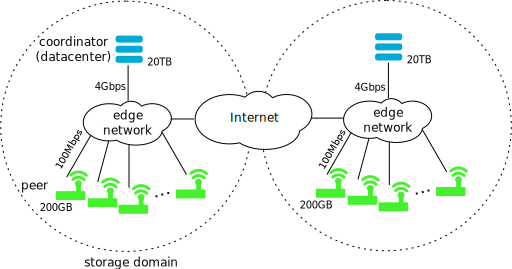
\includegraphics[width=.9\textwidth]{inputs/img/evaluation_scheme}
  \caption{Evaluation scenario.}
  \label{fig:evaluation_scenario}
\end{figure}

Our evaluation scenario (Figure~\ref{fig:evaluation_scenario}) includes 4002 nodes, arranged across two storage domains. There are one coordinator and 2000 peers per storage domain. Storage and network capacities differ according to the device role. Coordinators have 20TB of storage capacity and full-duplex access link of 4Gbps. Peers contribute 200GB each, equipped with 100Mbps full-duplex links. Note that the two coordinators contribute with a small fraction of aggregate edge resources, i.e. 5\% of the storage capacity and only 2\% of the total network capacity. This draws our attention to the performance of replication schemes towards peers resource allocation. We assume only 1\% peers' storage is available for caching additional replicas, namely 2GB.

We implemented and evaluate this work using simulation. To this end, we developed a simulation tool on top of PeerSim~\cite{p2p09-peersim} to implement storage domains in edge network and bandwidth scheduling.Our design focus on network's resource allocation accuracy for simulating bitrate enforcement and concurrent videos views properly.  Design and implementations details of our tools to simulate network resource scheduling are available in our previous work~\cite{silvestre2010most}. We have performed our simulations using servers equipped with Intel Xeon E5450 3.00 GHz, and a RAM of 4GB. 

\subsection{Comparable Replication Schemes}
\label{subsec:methodology_replication_schemes}

We compare WiseReplica with two other schemes.

\noindent
{\bf Non-collaborative caching}. Adaptive replication schemes based on non-collaborative caching, such as those that uses Least Recent Used (LRU) algorithm, are easy to implement and deploy. A new replica is created in a peer whenever a user requests to view a video. LRU replacement is enforced regarding the static percentage of the local storage capacity for caching of 1\%.

\noindent
{\bf Oracle-like collaborative caching}. This is an idealized benchmark case. Here, we assume a peer-assisted VoD system deployed in a network that runs a deadline-aware transport protocol, similar to Wilson \emph{et al.}\cite{d3_sigcomm2011} work. Based on our previous work with AREN~\cite{silvestre_aren_icpads12}, an adaptive replication scheme for edge networks, we implemented a benchmark replication scheme that relies on bandwidth reservation and collaborative
caching to provide an adaptive number of replicas for videos. We replicate videos according to aggregate network usage by enforcing a low and high thresholds. This makes the video replication a function of bandwidth reservation, and ensures that network and storage provision follows video demand properly, as depicted in Figure~\ref{fig:oracle_like}. Per video, we consider two percentage thresholds for aggregate network usage: $P_{min}$ and $P_{max}$. Our replication strategy works as follows. A video $v$ that has $N$ replicas in peers with network capacity of $b$ requires more replicas if the current bandwidth reservation $U(v) > P_{max} \sum_{i=1}^N b$. Similarly, if $U(v) < P_{min} \sum_{i=1}^N b$, replicas can be deleted. Otherwise, keep the replication degree. Although this empirical approach is hard to be adopted in a real deployment, our previous results~\cite{silvestre_aren_icpads12} suggest that it allows us to achieve near-optimal results, preventing \emph{all} SLA violations, enhancing network usage and decreasing storage usage dramatically.  

\begin{figure}
  \centering
     
\includegraphics[width=.6\textwidth]{inputs/img/oracle_like}
  \caption{Oracle-like bandwidth management for a video, illustrating aggregate bandwidth for $N$ replicas and $b$ available bandwidth, bandwidth reservation (bandwidth usage) and thresholds ($P_{min}$ and $P_{max}$).}
  \label{fig:oracle_like}
\end{figure}


\subsection{Collecting the Datasets for Learning}
\label{subsec:methodology_training_dataset}

To perform rank predictions of Internet videos, we need training datasets from which we can learn the behaviour of video demand in peer-assisted VoD systems. In this section, we explain the methodology to gather data for these predictions. 

The training dataset of our prediction model comes from measurements of the request arrival process on per-assisted VoD systems, as described in Subsection~\ref{subsec:learning_model_details}. Each line of our training dataset has 11 values, 10 input measurements about a video current state, and a rank position. Although, the datasets evaluated in this work were synthetically collected by performing simulations with the Oracle-like benchmark replication approach (detailed in Subsection~\ref{subsec:methodology_replication_schemes}), similar datasets can be collected from monitoring systems of running CDN systems.

In this work, Oracle-like benchmark replication approach (Subsection~\ref{subsec:methodology_replication_schemes}) represents the near-optimal way to serve VoD service according to video encodings and popularity, whose functioning we are very interested in learning. In this empirical approach, a video requires additional replicas only if there exists a certain number of concurrent accesses, where concurrence is measured by checking a high threshold of the current reserved bandwidth, as detailed in Subsection~\ref{subsec:methodology_replication_schemes}. We assume that popular videos are those that have additional replicas during its lifetime. Since Internet videos popularity distribution follows a Zipf-like distribution~\cite{popularity_prediction_2010}, concurrent access are rare events as well as popular videos classified by this approach, thus it provides a quite fair approach to identify popular videos. 

Raw data from Oracle-like technique permits easily distinguishing between two ranking positions only, non-popular and popular videos, i.e. requests to non-popular videos are all those that do not trigger any replica creation, or those that resulted in deletions. However, there is a lack of information about different ranking positions of popular videos. Hence, depending on the frequency of replica creation, we add information to requests to popular videos classifying them in popular, very popular, or viral. To define these three levels of \emph{hotness}, we run simulations with YouTube traces, collected the distribution of replicas creation in milliseconds, and split it in three nearly equal parts by observing the 66-percentile and 33-percentile inter-creation time for new replicas. This means that the higher is the frequency of replica creation, the hotter is the video, and the higher is the ranking position. Now, collected data suit model's definitions well. 
